\chapter{Implementácia syntetizátora}

Pre implementáciu syntetizátora som si vybral jazyk C++ a vývojové prostredie Microsoft Visual Studio 2005. Do projektu bolo potrebné pridať súbory frameworku VST SDK. Pri implementácii som rozložil funkcionality syntetizátora do rôznych tried, ale z dôvodu nezlučiteľnosti s požiadavkami na čo najmenšiu záťaž procesora som neaplikoval niektoré princípy objektovo orientovaného programovania.

Základ syntetizátora pre rozhranie VST je trieda zdedená z triedy AudioEffectX. V mojej implementácii sa táto trieda volá MirSynth. Prvá vec, ktorú bolo nutné implenmentovať, je globálna funkcia \emph{createEffectInstance}, ktorá má za úlohu vytvoriť inštanciu syntetizátora a vrátiť smerník na ňu.

VST SDK vyžaduje implementáciu mnohých metód pre rôzne funkcie komunikácie s hostom. Sú to metódy pre komunikáciu ohľadom parametrov, systémových nastavení a programov.



\begin{figure}[h]
\centering
\resizebox{10cm}{!}{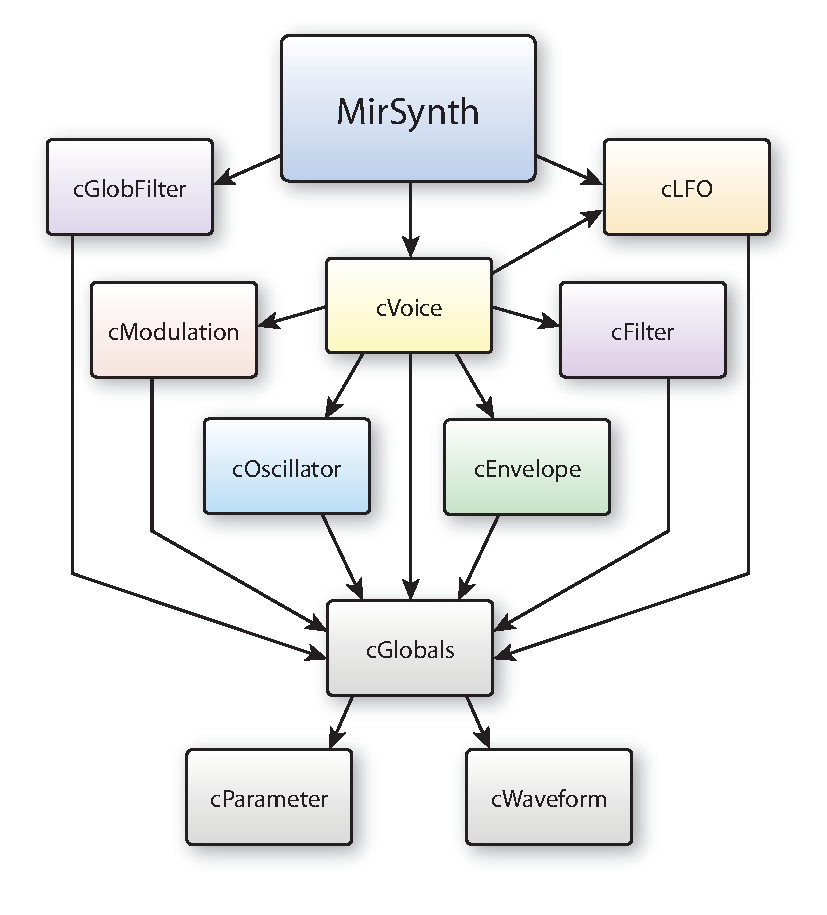
\includegraphics{classes}}
\caption{\label{obr11} Triedy syntetizátoru}
\end{figure}

\section{Popis tried}

Jadro syntetizátora pozostáva z jedenástich tried. 
\begin{description}
\setlength{\itemsep}{-0.5ex}
\item[MirSynth] -- je hlavná trieda zdedená z triedy AudioEffectX frameworku VST SDK. VST SDK vyžaduje implementáciu mnohých metód pre rôzne funkcie komunikácie s hostom. Sú to metódy pre komunikáciu ohľadom parametrov, systémových nastavení, programov a samotného spracovania udalostí a zvuku.
\item[cVoice] -- predstavuje jeden hlas v polyfónii. Tento hlas obsahuje oscilátory, obálky, nízkofrekvenčné oscilátory, filtre a modulátor. Všetky operácie na úrovni hlasu sa vykonávajú v rámci tejto triedy.
\item[cOscillator] -- predstavuje oscilátor.
\item[cFilter] - predstavuje filter.
\item[cGlobFilter] -- globálny filter -- trieda MirSynth vlastní dve inštancie tohto filtra. Je určený na odfiltrovanie spodných nepočuteľných frekvencií. Má pevne nastavené parametre -- hraničná frekvencia je 20~Hz, rezonancia je nulová. Tieto filtre sú dva v sérii kvôli väčšej strmosti filtrovania.
\item[cEnvelope] -- predstavuje obálku.
\item[cLFO] -- predstavuje nízkofrekvenčný oscilátor.
\item[cModulation] -- predstavuje modulátor.
\item[cGlobals] -- je trieda určená na sprostredkúvanie globálnych premenných ostatným triedam. Okrem iného vlastní aj inštanciu triedy cWaveform pre generovanie vĺn oscilátormi a nízkofrekvenčnými oscilátormi. Vlastní aj pole inštancií triedy cParameter pre uloženie aktuálnych parametrov.
\item[cParameter] -- je trieda vytvorená na uloženie hodnoty a vlastností parametrov. Táto trieda poskytuje aj textové interpretácie vlastností parametrov.
\item[cWaveform] -- trieda určená na prácu s vlnovými priebehmi. Má metódy na čítanie a interpolovanie vzoriek z tabuliek vĺn pre oscilátory aj pre nízkofrekvenčné oscilátory.
\end{description}

Pre generovanie tabuliek vĺn priebehov oscilátora som si vytvoril jednoduchú aplikáciu v jazyku C\#, ktorá vygenerovala celú tabuľku pre konkrétny priebeh a uložila vlnu do binárneho súboru. Zmenou vzorcov som vypočítal aj tabuľky ostatných priebehov. Tie som následne pridal do projektu ako resources.

\section{Popis významných operácií}

\subsection{Metóda \emph{processReplacing}}

Metóda \emph{processReplacing} je virtuálna metóda určená na spracovanie zvuku. Keď host volá túto metódu, očakáva od syntetizátora zvukový výstup.
Nasledujúci pseudokód opisuje fungovanie tejto metódy v mojej implementácii:

\begin{Verbatim}[fontsize=\relsize{-1.5}]
	01 vynuluje sa buffer
	02 interpolujú sa zmeny parametrov
	03 vypočítajú sa hodnoty globálnych LFO
	04 pre všetky hlasy polyfónie sa vykoná
		05 ak hlas hrá, vypočíta sa jeho vzorka a pripočíta sa k bufferu
	06 buffer sa vyfiltruje globálnymi filtrami
	07 buffer sa pošle na výstup
\end{Verbatim}

Pre prípad, že je veľkosť bloku väčšia ako 1 vzorka, tento kód sa vykonáva pre každú vzorku.

\subsection{Výpočet vzorky hlasu}

Výpočet vzorky hlasu prebieha v metóde \emph{getSample} triedy \emph{cVoice} nasledovne:

\begin{Verbatim}[fontsize=\relsize{-1.5}]
	01 vynuluje sa buffer
	02 vykonajú sa modulácie
	03 ak hlas hrá, vykoná sa:
		04 vypočítajú sa hodnoty obálok
		05 vypočítajú sa hodnoty LFO
		06 posunú sa fázy oscilátorov
		07 vypočítajú sa vzorky oscilátorov a pripočítajú sa k bufferu
	08 hodnota bufferu sa filtruje
	09 buffer sa posiela na výstup	
\end{Verbatim}

Posun fázy oscilátorov a výpočet ich hodnôt sú oddelené operácie, pretože kvôli synchronizácii je nutné najskôr vypočítať fázy všetkých štyroch oscilátorov, až potom počítať hodnoty vzoriek.

\subsection{Spracovanie MIDI udalostí}

Syntetizátor reaguje na MIDI udalosti nasledovne:

\begin{description}
\setlength{\itemsep}{-0.5ex}
\item[NOTE ON]: Ak je v poli hlasov hlas, ktorý nehrá, spustí sa s parametrami udalosti (nota, velocity). Ak hrajú všetky hlasy, reštartuje sa s novými parametrami ten najstarší.
\item[NOTE OFF]: Ak je v poli hlasov hlas, ktorý hrá príslušnú notu, hlas sa zastaví.
\item[CC]: Zmena MIDI ovládača sa zaznamená do poľa hodnôt MIDI ovládačov.
\item[AFTERTOUCH]: Zmena hodnoty sa zaznamená do pamäte.
\item[PITCH-WHEEL]: Zmena hodnoty sa zaznamená do pamäte.
\end{description}

O spracovanie udalostí sa stará metóda \emph{processEvents} triedy \emph{MirSynth}.

\subsection{Spustenie a zastavenie hlasu}

Spustenie hlasu vykonáva metóda \emph{playNote} triedy \emph{cVoice}.

\begin{Verbatim}[fontsize=\relsize{-1.5}]
	01 nastaví sa nota, velocity, poradové číslo noty
	02 resetujú sa oscilátory, LFO, obálky a filtre
	03 nastaví sa indikátor hrania noty na true
\end{Verbatim}

Zastavenie hlasu má na starosti metóda \emph{stopNote} triedy \emph{cVoice}. Tá uvedie obálky do fázy RELEASE. Po klesnutí všetkých hodnôt obálok na nulu sa 
nastaví indikátor hrania noty na hodnotu \emph{false}.

\section{Optimalizácia kódu}

Výkon procesora je veľmi drahým zdrojom pri práci so zvukom. Aby bolo zaručené neprerušené generovanie a spracovanie zvukového signálu v reálnom čase, špička záťaže procesora by nikdy nemala vystúpiť na hodnotu 100\%. Okrem toho, aj keby záťaž syntetizátora bola dosť nepatrná, aj tak je dôležité optimalizovať jeho kód, pretože pri práci s hudbou a zvukom sa zvykne používať veľké množstvo syntetizátorov a efektov súčasne.

V priebehu programovania syntetizátora som narazil na problémy s neprípustne vysokou záťažou procesora. Zmenou nastavení kompilátora, vypnutím všetkých funkcií pre ladenie (debugging), zapnutím optimalizácií kompilátora a zapnutím podpory pre inštrukcie SSE2\newfootnote{SSE2 je inštrukčná sada zavedená firmou \emph{Intel} zameraná hlavne na efektívnejšiu floating-point aritmetiku. SSE2 podporujú procesory \emph{Intel Pentium 4} a novšie a procesory \emph{AMD Opteron} a novšie.} som znížil zaťaženie procesora asi na desatinu pôvodnej hodnoty. Keďže staršie počítače nepodporujú inštrukčnú sadu SSE2, rozhodol som sa skompilovať dve nezávislé verzie, s podporou a bez podpory SSE2.

V syntetizátore prebieha mnoho operácií niekoľkostotisíckrát za sekundu. Napríklad pre vzorkovaciu frekvenciu 96\,000~Hz sa počíta vzorka oscilátora pre každý stereo hlas 96\,000 x 2 x 4 = 768\,000-krát. Pri súčasnom hraní viacerých nôt, ktorých môže byť až desať, je to potom násobok tejto hodnoty. Z toho vyplýva, že aj ušetrenie niekoľko málo cyklov procesora v operácii môže výrazne ovplyvniť záťaž procesora.

Po dlhšom skúmaní náročností jednotlivých operácií \cite{b07} som v zdrojovom kóde identifikoval a optimalizoval nasledovné problémy:

\begin{description}
\setlength{\itemsep}{-0.5ex}
\item[Pretypovanie float na int] -- je vysoko neefektívna operácia, ak nie je použitá inštrukčná sada SSE2. Typický čas konverzie je 40 cyklov procesora. Pre túto konverziu som použil funkciu \emph{lrintf}\newfootnote{Funkcia je opísaná v dokumente \cite{b07}.}, ktorá je čisto assemblerová.
\item[Neefektívne používanie typov] -- zbytočné miešanie typov float a double, použitie \emph{double} pri násobení alebo delení, kde pre požadovanú presnosť postačuje typ \emph{float}. Tento problém je potrebné riešiť logickým prehodnotením a preusporiadaním operácií.
\item[Viacnásobné rovnaké výpočty] -- je veľmi neefektívne, ak sa pre každú vzorku počíta nejaká hodnota, ktorá sa mení len pri určitých udalostiach. Napríklad, ak nastane zmena určitého parametra a pre výpočty vzoriek používam jeho zložitý prepočet (napríklad mocnina), je potrebné si túto hodnotu hneď prepočítať a vo výpočtoch už pracovať s touto hodnotou.
\item[Redundantné výpočty] -- sú výpočty, ktoré je možné matematickými úpravami zmeniť tak, že sa zmenší ich výpočtová zložitosť. Napríklad:
\begin{equation*}
10^a \times 10^b \Rightarrow 10^{a+b}
\end{equation*}
V uvedenom príklade sa namiesto dvoch mocnín a jedného násobenia vykonáva len jedna mocnina a jedno sčítanie\footnote{Sčítanie je pre procesor oveľa jednoduchšia operácia ako násobenie.}.
Kompilátory sú často schopné zjednodušiť niektoré základné typy redundancie, ale pri mierne zložitejších výpočtoch je zjednodušovanie ponechané na programátora.
\item[Delenie] - delenie čísel je ďalšia neefektívna operácia. V prípadoch, keď je deliteľ konštantný pre viacero operácií, je efektívnejšie si predpočítať jeho obrátenú hodnotu, a tou v ďalších krokoch násobiť.
\item[Príliš veľa rozhraní] - prechody rozhraniami objektov a zapuzdrenie môžu znamenať výrazný pokles efektivity výpočtov. Ja som sa rozhodol pre prístup k atribútom objektov využívať priame smerníky.
\item[Reťazenie závislosti za sebou nasledujúcich operácií] -- moderné procesory disponujú paralelným počítaním niektorých kombinácií inštrukcií. Táto funkcionalita sa nazýva \emph{Out of order execution}. Aby ale tento princíp vykonávania kódu bol efektívny, je dôležité, aby po sebe nasledujúce výpočty neboli na sebe závislé.
\item[Denormalizácia] - denormalizované čísla sú floating-point čísla, ktoré sú tak blízko nuly, že na ich vyjadrenie nepostačuje bežný spôsob zápisu v pamäti. Tieto čísla používajú vlastný spôsob zápisu a operácie, kde je aspoň jeden operand denormalizovaný, sú extrémne pomalé, obzvlášť na procesoroch Intel. Všetky regeneratívne algoritmy sú náchylné k denormalizácii. V mojej implementácii IIR filtra spôsobuje spätná väzba náchylnosť k denormalizácii. 
Na ošetrenie náchylných hodnôt som použil metódu pripočítania a odpočítania veľmi malej konštanty, ktorá je ale dosť veľká na to, aby pri spočítaní s denormalizovanou hodnotou túto hodnotu pohltila. Po odpočítaní sa pôvodne denormalizovaná hodnota rovná nule. Pri normálnych hodnotách nenastane žiadna zmena. Pre túto konštantu som určil hodnotu $1 \times 10^{-18}$.
\end{description}

\section{Implementácia GUI}
Grafické používateľské rozhranie je implementované pomocou multiplatformnej knižnice VSTGUI. Knižnica VSTGUI je súčasťou balíka VST SDK. Táto knižnica poskytuje základné triedy a komponenty na vytvorenie grafického rozhrania.

Použité triedy:

\begin{description}
\setlength{\itemsep}{-0.5ex}
\item[cMirEditor] -- samotné grafické rozhranie, 
\item[CAnimKnob] -- potenciometer parametra,
\item[CParamDisplay] -- displej s hodnotou parametra, 
\item[cMultiStateButton] -- viacpolohové prepínacie tlačidlo, 
\item[cEnvDisplay] -- displej obálky, 
\item[cModAmtKnob] -- ovládač miery modulácie, 
\item[cModSelect] -- výberové menu pre zdroje a ciele modulácie, 
\item[cSyncButton] -- tlačidlo pre synchronizáciu oscilátora. 
\end{description}

Na prípravu grafických materiálov som použil program Adobe Photoshop. Pre animáciu potenciometrov bolo nutné vytvoriť jeden obrázok, v ktorom boli vertikálne pospájané všetky možné polohy potenciometra. Pre bežné parametre to bolo 128 polôh a pre mieru modulácie 201 polôh. Ručné vytváranie týchto materiálov by bolo nesmierne náročné na čas. Ja som riešil tento problém automatizovaním Photoshopu použitím javaScriptu.

Druhý významný problém v priebehu implementácie bolo vytvorenie displeja pre obálky, a vykresľovanie ich aktuálneho tvaru. VSTGUI síce poskytuje základné funkcie pre kreslenie čiar, avšak nemá implementáciu antialiasovania čiar pre platformu Windows. Preto som musel implementovať funkcie pre antialiasované čiary sám. Na to som použil veľmi efektívny algoritmus \emph{Wu}\newfootnote{Wu je algoritmus pre vykresľovanie antialiasovaných tvarov. Je nazvaný podľa svojho vynálezcu Xiaolina Wu. \cite{b10}}.

\section{Testovanie}

Testovanie syntetizátora som robil priebežne počas celej implementacie spolu s ďalším testerom. Na jeho procesore Intel Pentium 4 taktovanom na 3,7~GHz syntetizátor vykazoval nadmernú záťaž. Ja som testoval na procesore Intel Core2 Quad na 2,66~GHz a~na AMD Athlon 2800 taktovanom na 1,6~GHz. Na týchto konfiguráciách bola záťaž procesora prijateľná, takže som nebol schopný overiť a identifikovať pôvod zvýšenej záťaže na procesore Pentium. 
 Finálnu verziu syntetizátora som nechal testovať rovnako, ako boli testované syntetizátory v kapitole \ref{sucasnystav}. Výsledky sú zhodnotené v~nasledujúcej kapitole.

